\section{Related Work}
\label{sec:bg}



%%%%%%%%%%%%%%%%%%%%%%%%%%%%%%%%%%%%%%%%%%%

\para{Optimization-based upsampling.} \
To upsample a point set, a pioneering method by Alexa~\etal~\cite{alexa2003computing} inserts points at Voronoi diagram vertices in the local tangent space.
%%
Later, Lipman~\etal~\cite{lipman2007parameterization} introduced the locally optimal projection (LOP) operator to resample points and reconstruct surfaces based on an $L_1$ norm.
%, which is able to produce plausible results, even under noise and outliers.
%%
Soon after, Huang~\etal~\cite{huang2009consolidation} devised a weighted LOP with an iterative normal estimation to consolidate point sets with noise, outliers, and non-uniformities.
Huang~\etal~\cite{huang2013edge} further developed a progressive method called EAR for edge-aware resampling of point sets.
%
Later, Wu~\etal~\cite{wu2015deep} proposed a consolidation method to fill large holes and complete missing regions by introducing a new deep point representation.
%%
Overall, these methods are {\em not\/} data-driven; they heavily rely on priors,~\eg, the assumption of smooth surface, normal estimation,~\etc

\begin{figure*}[t]
	\centering
	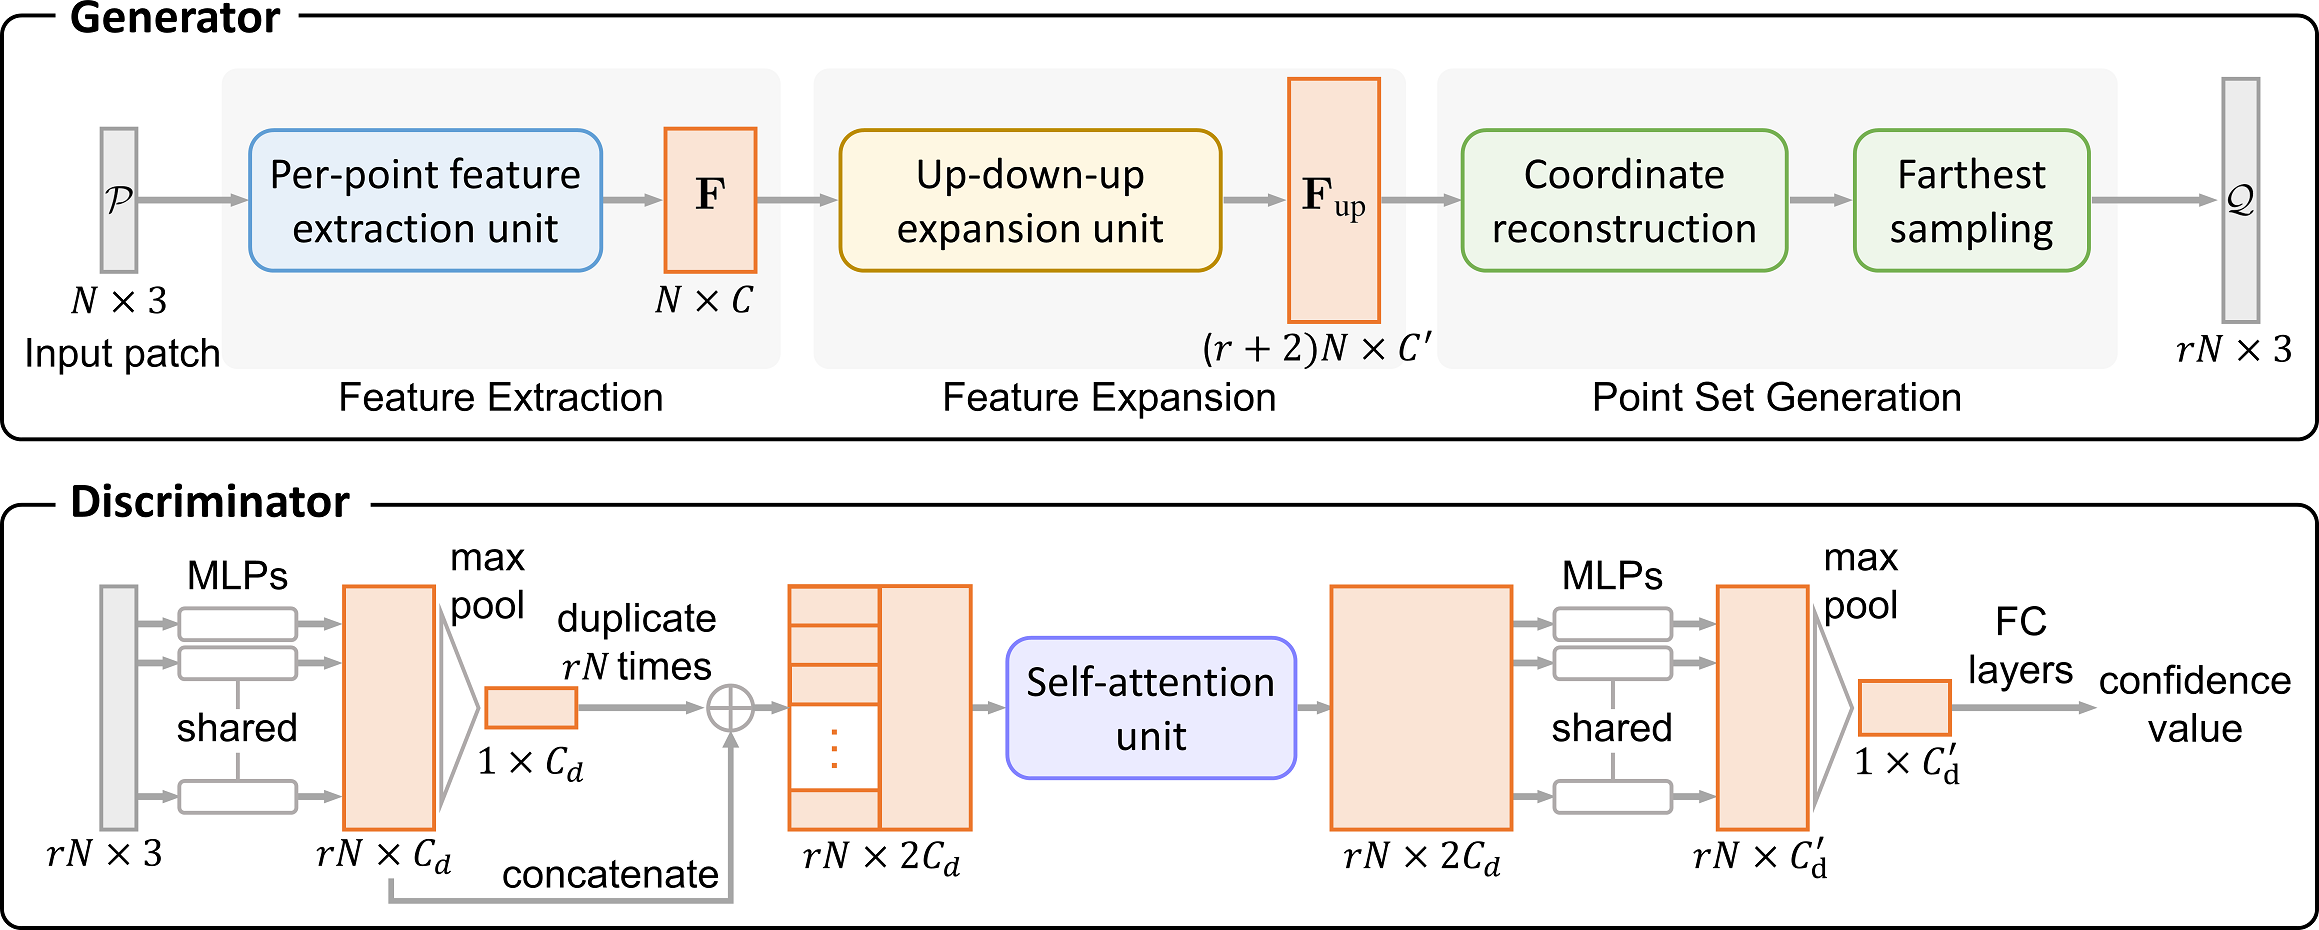
\includegraphics[width=0.88\linewidth]{framework}
	\caption{Overview of PU-GAN's generator and discriminator architecture.
Note that $N$ is the number of points in input $\mathcal{P}$; $r$ is the upsampling rate; and $C$, $C'$, $C_d$, and $C_d'$ are the number of feature channels that are 480, 128, 64, and 256, respectively, in our implementation.}
	\label{fig:framework}
	\vspace*{-2mm}
\end{figure*}

%%%%%%%%%%%%%%%%%%%%%%%%%%%%%%%%%%%%%%%%%%%

\para{Deep-learning-based upsampling.} \
%\phil{XZ: a very short paragraph here to talk about and mention various works on deep feature learning on point cloud}
In recent few years, several deep neural networks have been designed to learn features directly from point sets,~\eg, PointNet~\cite{qi2016pointnet}, PointNet++~\cite{qi2017pointnet++}, SpiderCNN~\cite{xu2018spidercnn}, KCNet~\cite{shen2018mining}, SPLATNet~\cite{su2018splatnet}, PointCNN~\cite{li2018pointcnn}, PointConv~\cite{hua2017pointwise}, PointWeb~\cite{zhao2019pointweb}, DGCNN~\cite{wang2018dynamic}, \emph{etc}.
\rh{Different from point completion ~\cite{yuan2018pcn,gurumurthy2019high} which
generates the entire object from partial input, point cloud upsampling tends to improve the point distribution uniformity within local patches.}
Based on the PointNet++ architecture, Yu~\etal~\cite{yu2018pu} introduced a deep neural network PU-Net to upsample point sets.
PU-Net works on patches and expands a point set by mixing-and-blending point features in the feature space.
Later, they introduced EC-Net~\cite{yu2018ec} for edge-aware point cloud upsampling by formulating an edge-aware joint loss function to minimize the point-to-edge distances.
%regressing a point-to-surface distance and minimizing the point-to-edge losses.
%
Very recently, Wang~\etal~\cite{yifan2018patch} presented a multi-step progressive upsampling (MPU) network to further suppress noise and retain details.
%while He~\etal~\cite{he2019geonet} developed a geodesic neighborhood estimation network GeoNet by fusing the learned geodesic-aware representations into PU-Net.
%
In this work, we present a new method to upsample point clouds by formulating a GAN framework, enabling us to generate higher-quality point samples with completion and uniformity.

%\phil{What is he2019geonet? If we mention it here like this, we have to compare with it quantitatively}



%%%%%%%%%%%%%%%%%%%%%%%%%%%%%%%%%%%%%%%%%%%

%\para{Deep feature learning on point sets.} \
%%
%The advent of fast 3D point cloud acquisition and rapid advances in 3D sensing encourage the development of deep feature learning on point sets.
%%
%Qi~\etal~\cite{qi2016pointnet} introduced the first deep learning network, PointNet, that consumes point sets directly; in particular, its variant PointNet++~\cite{qi2017pointnet++} uses a hierarchical feature learning architecture to capture both local and global geometry context.
%%
%Subsequently, many other networks were proposed for better feature embedding,~\eg, pointwise convolution~\cite{hua2017pointwise}, SpiderCNN~\cite{xu2018spidercnn}, PointGrid~\cite{le2018pointgrid}, KCNet~\cite{shen2018mining}, SPLATNet~\cite{su2018splatnet}, PointCNN~\cite{li2018pointcnn}, DGCNN with EdgeConv block~\cite{wang2018dynamic},~\etc.

\para{GAN-based 3D shape processing.} \
%\phil{(1) start this paragraph by describing the key advantage or strength of GAN over conventional CNN... this helps!}
%\phil{(2) can you shorten the contents below?}
Compared with the conventional CNN, the GAN framework makes use of a discriminator to implicitly learn to evaluate the point sets produced from the generator.
%avoid the need of explicitly designing a loss function to evaluate the network output.
%
Such flexibility particularly benefits generative tasks~\cite{ledig2017photo,isola2017image,zhang2017stackgan}, since we hope the generator can produce a rich variety of output patterns.
%it is often difficult to formulate a perfect loss function.
%\phil{did we get rid of an explicit supervision? if not, need to change the sentence as follows:}
%Such flexibility particularly benefits generative tasks\phil{cite some works on GAN here?}, where ...
%
%Compared with the conventional CNN, by using GAN, we do not need to explicitly design a loss function to evaluate the network output.
%This will undoubtedly bring lots of benefits to these generative-related tasks, because it is often difficult to design a perfect loss function in these tasks.

Recently, there are some inspiring works in applying GAN to 3D shape processing.
Most of them focus on generating 3D objects either from a probabilistic space~\cite{wu2016learning} or from 2D images~\cite{yang20173d,gwak2017weakly,smith2017improved}.
Moreover, Wang~\etal~\cite{wang2017shape} introduced a 3D-ED-GAN for shape completion given a corrupted 3D scan as input.
However, these methods can only consume 3D volumes as inputs or output shapes in voxel representations.
%
Achlioptas~\etal~\cite{achlioptas2018learning} first adapted the GAN model to operate on raw point clouds for enhancing the representation learning.
%superior reconstruction quality.
%However, they mainly focus on representation learning.
%\phil{can its network be adopted to point set upsampling? do we need to compare with this work?}
%
To the best of our knowledge, no prior works develop GAN models for point cloud upsampling.
%\phil{can we really say so, given~\cite{achlioptas2018learning} and the works here?}
%\xz{yes, we can. That work is totally different from us. It has no relationship to upsampling.}
